\chapter{Phase II: Design}\label{Design}

In der Design-Phase wurde die Architektur des Systems entworfen. Ausgehend von den Erkenntnissen der Analyse-Phase wurden zun�chst wichtige, grundlegende Entscheidungen gef�llt und schlie�lich ein Designklassen-Diagramm erstellt. F�r einige wichtige Operationen wurden au�erdem Sequenzdiagramme angefertigt, um weitere Einblicke in die Funktionsweise des Systems zu gewinnen. F�r die Anbindung der GUI wurde ein eigenst�ndiges Framework entwickelt, f�r das es ein eigenes Designklassen-Diagramm gibt.

\section{Grundlegende Entscheidungen}\label{decisions}	
Eine Anforderung an das System war die Unabh�ngigkeit von \Horde\ und der Anwendung des Benutzers. Bereits in der Design-Phase musste daher sichergestellt werden, dass die Implementierung keine �nderungen an \Horde\ oder der Benutzeranwendung voraussetzt. Die \emph{Use Cases} fordern zus�tzlich, dass das System die Anwendung des Benutzers starten und beenden kann. Eine Client-Server-Architektur zwischen \DevEnv\ und Anwendung, welche  service-orientiert entworfen wurde, erf�llt diese Anforderungen. Was nun als Server bezeichnet wird, ist in diesem Fall allerdings nicht klar. F�r die \Horde-Anwendung spricht, dass sie die Daten h�lt, die von dem System ausgelesen und angezeigt werden. F�r das System spricht hingegen, dass es die ganze Zeit l�uft und die \Horde-Anwendung erst starten muss. Das Festlegen einer genauen Terminologie wird zus�tzlich durch den Einsatz eines DLL-\emph{Replacement}-Mechanismus erschwert. Die originale \Horde\ DLL wird durch eine modifizierte Version ersetzt, die alle \Horde-Funktionsaufrufe -- f�r die Anwendung v�llig transparent -- an die Original-DLL weiterleitet und intern noch zus�tzlichen Code ausf�hrt. Dadurch schleust das \DevEnv\ Code in die \Horde-Anwendung ein; das System l�uft sowohl server- als auch client-seitig. 

In den n�chsten Abschnitten wird nun folgende Terminologie verwendet: Mit "`\Horde-Anwendung"' ist die Anwendung des Benutzers gemeint, ohne DLL-\emph{Replacement}. "`Server"' bezeichnet den Code des \DevEnvs, der innerhalb des Prozesses der \Horde-Anwendung l�uft. "`Client"' oder "`Shell"' ist der Teil des Systems, der als eigenst�ndige Applikation lauff�hig ist und Server-Instanzen starten und beenden kann. 

\begin{figure}[ht]
\centering
%trim=l b r t  	This option will crop the imported image by l from the left, b from the bottom, r from the right, and t  from the top. Where l, b, r and t are lengths. 
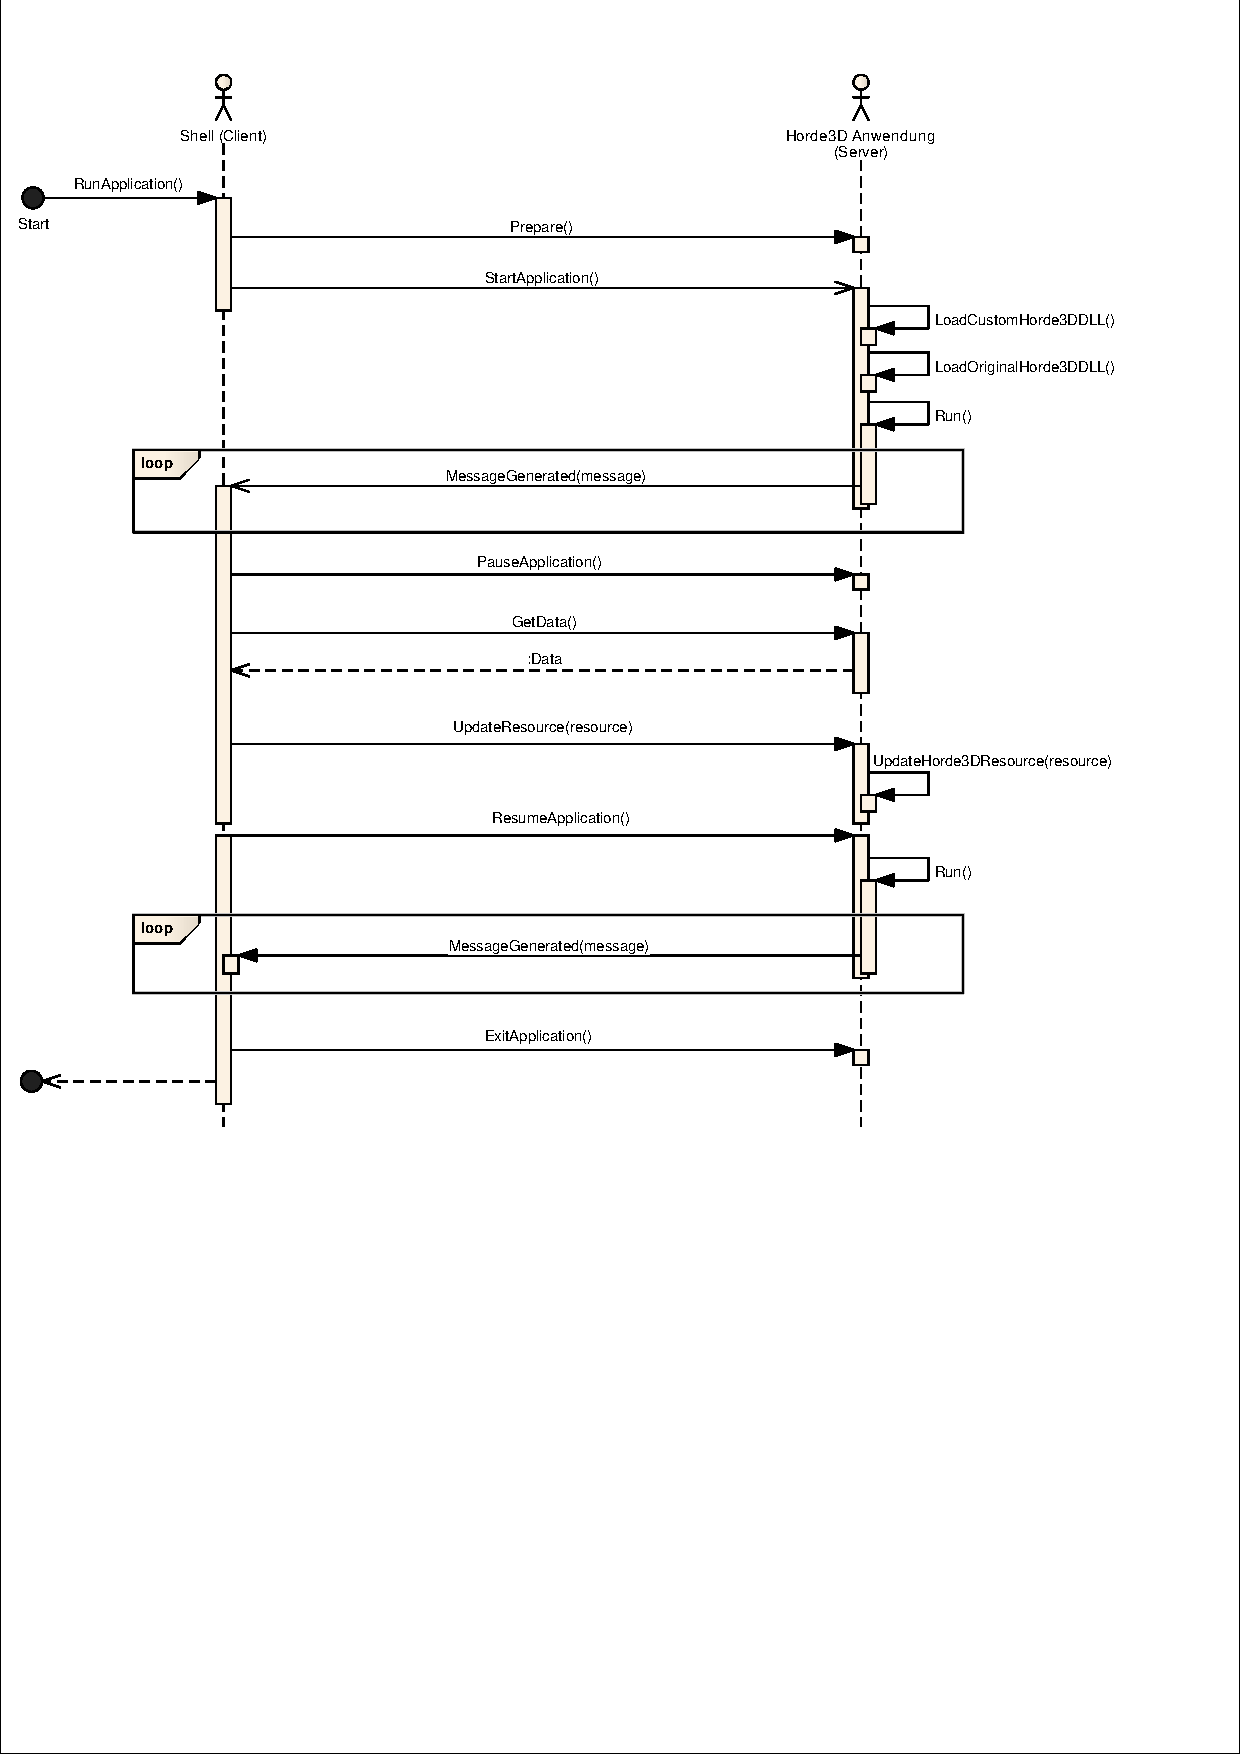
\includegraphics[trim = 3mm 100mm 15mm 12mm, clip, scale=0.7]{images/Prozess.pdf}
\caption{Interaktionen zwischen Client und Server an einem Beispiel}\label{fig:prozess}
\end{figure}

Abbildung~\ref{fig:prozess} verdeutlicht die Interaktionen zwischen Server und Client an einem Beispiel. Der Client wird dabei durch die Lebenslinie des linken Akteurs repr�sentiert, die rechte Lebenslinie repr�sentiert den Server. Die Shell f�hrt zun�chst ein paar vorbereitende Schritte durch -- unter anderem das DLL-\emph{Replacement} sowie einige Konfigurationsaufgaben -- und startet schlie�lich die \Horde-Anwendung. Anstelle der Original-DLL wird jedoch die modifizierte \Horde\ DLL geladen und initialisiert. W�hrend der Initialisierung wird schlie�lich die originale \Horde\ DLL in den Prozess geladen. Anschlie�end wird die Anwendung normal ausgef�hrt und alle von \Horde\ generierten Meldungen sofort an den Client geschickt.

Zu einem beliebigen Zeitpunkt weist der Benutzer die Shell an, die \Horde-Anwendung zu pausieren. Nun k�nnen alle relevanten Daten -- beispielsweise der aktuelle Zustand des Szenengraphs oder die derzeit bekannten Ressourcen -- aus dem Server ausgelesen werden. Anschlie�end wird eine Ressource ver�ndert und deren aktualisierte Daten wieder an den Server geschickt, der die entsprechende \Horde-Ressource aktualisiert. Danach wird die Anwendung fortgesetzt und beim Zeichnen die aktualisierte Ressource verwendet, bis die Shell den Server schlie�lich beendet.

\begin{figure}[ht]
\centering
%trim=l b r t  	This option will crop the imported image by l from the left, b from the bottom, r from the right, and t  from the top. Where l, b, r and t are lengths. 
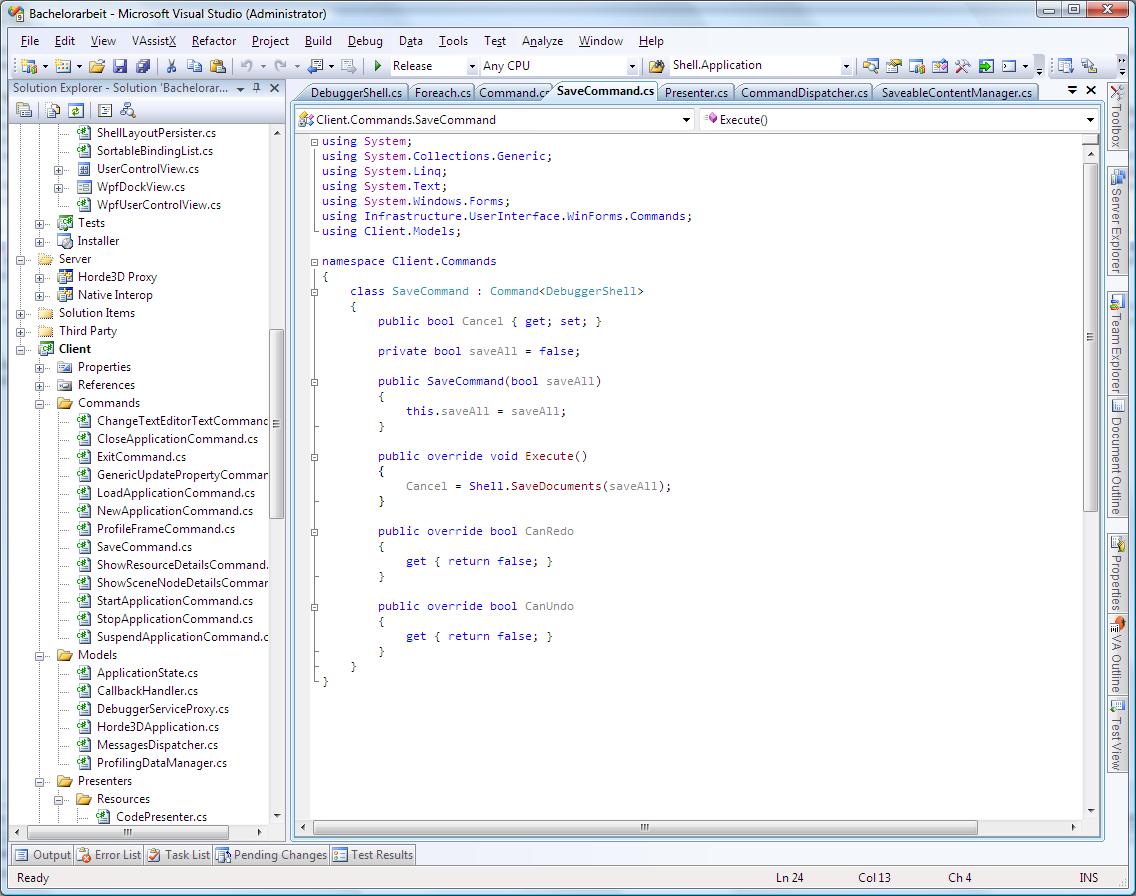
\includegraphics[scale=0.38]{images/VS.png}
\caption{Die grafische Benutzeroberfl�che von Visual Studio 2008}\label{fig:vs}
\end{figure}

Auch �ber die grafische Benutzeroberfl�che wurde bereits am Anfang der Design-Phase nachgedacht. Das \emph{User Interface} sollte sich an GUIs bekannter Entwicklungsumgebungen wie Visual Studio und Eclipse orientieren. Abbildung~\ref{fig:vs} verdeutlicht die geplante GUI am Beispiel von Visual Studio 2008: In der Mitte des \emph{Workspaces} werden mehrere Dokumente oder grafische Designer angezeigt. Oben gibt es die bereits von Windows bekannten Men�s und \emph{Toolbars}. An der rechten und an der unteren Seite sind verschiedene \emph{Tool Windows} versteckt, die erst beim Ber�hren mit der Maus sichtbar werden. Links ist das \emph{Solution Explorer Tool Window} "`angedockt"'. Die \emph{Tool Windows}, auch \emph{Dock Panes} genannt, k�nnen vom Benutzer frei positioniert sowie versteckt und wieder sichtbar gemacht werden. Es besteht auch die M�glichkeit, die \emph{Dock Panes} als eigenes Fenster (\emph{Floating Window}) �ber die Anwendung zu legen. Das vom Benutzer frei gew�hlte Layout wird gespeichert und beim Starten der Anwendung automatisch wiederhergestellt. 

Das \DevEnv\ wurde im Hinblick auf ein solches GUI-Design entworfen, da es weit verbreitet und bekannt ist und es dem Benutzer viele M�glichkeiten l�sst, die Oberfl�che an seine W�nsche und Vorlieben anzupassen. 

Zu Beginn der Design-Phase wurde auch entschieden, dass das System in \Csharp\ mit dem .NET Framework 3.5 Service Pack 1 implementiert wird. Dadurch ist das System zwar nur unter Windows lauff�hig, aufgrund der h�heren Produktivit�t gegen�ber einer Implementierung mit \C++ und Qt konnte bei der Entwicklung jedoch mehr Zeit in die eigentlich zu l�senden Probleme investiert werden. Diese Entscheidung wurde bereits zu diesem Zeitpunkt getroffen, damit schon in den Design-Artefakten .NET \emph{Properties} und \emph{Events} verwendet werden k�nnen, was die Darstellung erleichtert und verk�rzt. Da UML jedoch keine Unterst�tzung f�r diese Konzepte anbietet, wurden die entsprechenden UML-Attribute und -Operationen mit den Stereotypen \texttt{property} (\emph{Getter} und \emph{Setter} f�r Attribute), \texttt{event} (ein Ereignis, das auftreten kann) und \texttt{event property} (an diesem kann sich ein Objekt f�r ein \emph{Event} registrieren und deregistrieren) versehen.

All diese Entscheidungen hatten einen gro�en Einfluss auf den Gesamtentwurf des Systems. Deshalb war es wichtig zu �berpr�fen, ob die vorgestellten Konzepte �berhaupt wie geplant umsetzbar sind. Vor dem Entwurf der Design-Dokumente wurde daher ein Prototyp entwickelt, der die Machbarkeit der Konzepte �berpr�fte und als durchf�hrbar best�tigte.
\section{Angewandte Entwurfsmuster}
In der Softwareentwicklung gibt es f�r ein spezielles Architektur-Problem oftmals mehrere m�g\-liche L�sungswege. Diese sind je nach Situation besser oder schlechter geeignet. Eine der wichtigsten F�higkeiten eines Softwarearchitekten ist es daher, unterscheiden zu k�nnen, was f�r ein gegebenes Problem derjenige L�sungsansatz ist, der zum bestm�glichen Design f�hrt \cite[S. 4]{cpp}. Auf der anderen Seite gibt es in der Softwareentwicklung eine Vielzahl an wiederkehrenden Entwurfsproblemen, f�r die es bew�hrte L�sungsschablonen gibt. Die Schablonen, \emph{Design Patterns} oder Entwurfsmuster genannt, stellen eine allgemeine Vorlage zur Probleml�sung dar, die nur noch auf den spezifischen Kontext des Problems angepasst werden muss. Gut strukturierte, objekt-orientierte Softwarearchitekturen verwenden eine Vielzahl an unterschiedlichen \emph{Design Patterns} \cite{gangOfFour}.

Beim Design des \DevEnvs\ wurden verschiedene \emph{Design Patterns} angewandt, die im folgenden kurz vorgestellt werden. Bei der Vorstellung des Systemdesigns wird immer wieder auf die Verwendung der \emph{Patterns} zur L�sung eines Design-Problems hingewiesen.

\subsection{General Responsibility Assignment Software Patterns}
F�r die Zuweisung der Verantwortlichkeiten auf die einzelnen Klassen wurden einige der \emph{General Responsibility Assignment Software Patterns} verwendet \cite{grasp}. Da die \emph{Patterns} aber die Grundlage f�r objekt-orientierte Entw�rfe bilden und somit vielfach angewandt wurden, wird auf eine Instanziierung eines GRAS Entwurfsmuster im Designmodell nicht hingewiesen. Im folgenden seien die verwendeten \emph{GRAS Patterns} aber kurz vorgestellt:

\begin{itemize}
	\item \textbf{Expert:} \emph{Expert} ist das allgemeinste \emph{Pattern}. Diejenige Klasse sollte die Verantwortlichkeit erhalten, die alle ben�tigten Informationen daf�r besitzt.
	\item \textbf{Creator:} Das \emph{Creator Pattern} gibt Hinweise darauf, welche Klasse eine Instanz einer anderen Klasse erzeugen sollte. Ein Objekt $B$ sollte ein Objekt $A$ erzeugen, wenn beispielsweise $B$ eine Aggregation von $A$ ist, oder $B$ die ben�tigten Initialisierungsdaten f�r $A$ besitzt.
	\item \textbf{Low Coupling:} Mit Kopplung bezeichnet man das Ma� der Abh�ngigkeit einer Klasse von anderen Klassen. Eine niedrige Kopplung ist eines der wichtigsten Ziele von gutem objekt-orientierten Design, da es die Wiederverwendbarkeit erh�ht und auch die Verst�ndlichkeit und Wartbarkeit des Codes verbessert.
	\item \textbf{High Cohesion:} Die Koh�sion einer Klasse bezeichnet den semantischen Zusammenhang der Verantwortlichkeiten einer Klasse. Eine Klasse sollte m�glichst wenige verschiedene Aufgaben enthalten, um eine hohe Koh�sion zu erreichen. Dadurch werden die Klassen kleiner, die Verantwortlichkeiten einer Klasse genauer definiert und der Code damit insgesamt besser wartbar, verst�ndlich und wiederverwendbar. Jedoch steht das \emph{High Cohesion Pattern} im Widerspruch zu \emph{Low Coupling}. Beim Softwareentwurf muss daher eine angemessene Balance gefunden werden.
	\item \textbf{Polymorphismus:} Polymorphismus ist ein grundlegendes \emph{Pattern} der objekt-orientier\-ten Entwicklung, das von allen modernen objekt-orientierten Programmiersprachen direkt unterst�tzt wird. Durch die Verwendung von virtuellen und polymorphen Funktionen kann das Verhalten abh�ngig vom konkreten Typ der Klasse(n) ge�ndert werden.
	\item \textbf{Pure Fabrication:} Mit \emph{Pure Fabrication} bezeichnet man die Einf�hrung von Design-Klassen, die im Design eine spezielle Aufgabe �bernehmen, im Konzeptmodell aber nicht vorhanden sind.
\end{itemize}

\subsection{Gang of Four Design Patterns}
Der Entwurf des \DevEnvs\ verwendet einige der bekannten und oft eingesetzten \emph{Design Patterns} der \emph{Gang Of Four} \cite{gangOfFour}. Diejenigen dieser Entwurfsmuster, die f�r das Systemdesign eingesetzt wurden, seinen hier kurz erl�utert; an den entsprechenden Stellen wird auf ihre genaue Verwendung hingewiesen.

\begin{itemize}
	\item \textbf{Composite:} Das \emph{Composite Pattern} \cite[S. 163ff]{gangOfFour} f�gt mehrere Objekte in einer Baumstruktur zusammen, um eine Teil-Ganzes-Hierarchie zu repr�sentieren. Ein Knoten muss nicht unterscheiden, ob eines seiner Kinder ein Blatt oder wiederum ein Knoten mit weiteren Kindern ist. Primitive Objekte und Beh�lter k�nnen also uniform behandelt werden.
	\item \textbf{Facade:} Das \emph{Facade Pattern} \cite[S. 185ff]{gangOfFour} fasst verschiedene Interfaces unter einem gemeinsamen, einfacher benutzbaren Interface zusammen. Damit werden Komplexit�t und Abh�ngigkeiten reduziert, und somit das System besser wartbar.
	\item \textbf{Command:} Beim \emph{Command Pattern} \cite[S. 233ff]{gangOfFour} wird eine Operation durch ein Objekt gekapselt. Durchgef�hrte Operationen k�nnen parametrisiert und protokolliert werden. Dadurch wird es m�glich, Operationen sp�ter r�ckg�ngig zu machen.
	\item \textbf{Observer:} Das \emph{Observer Pattern} \cite[S. 293ff]{gangOfFour} wird direkt von zwei \Csharp-Sprachfeatures unterst�tzt: \emph{Delegates} und \emph{Events}. Objekte k�nnen einen speziellen \emph{Event Handler Delegate} f�r ein \emph{Event} eines (anderen) Objekts registrieren. L�st das Objekt das Ereignis aus, werden alle registrierten \emph{Delegates} automatisch ausgef�hrt. Das Objekt muss daf�r nicht wissen, welche Objekte oder ob �berhaupt Objekte an diesem Ereignis interessiert sind. Mit Hilfe dieses \emph{Patterns} kann eine \emph{One-To-Many}-Beziehung definiert werden, ohne zus�tzliche Abh�ngigkeiten einzuf�hren.
	\item \textbf{Singleton:} Das \emph{Singleton Design Pattern} \cite[S. 127ff]{gangOfFour} stellt sicher, dass es nur eine Instanz einer Klasse geben kann. F�r diese Instanz gibt es einen einzigen, globalen Zugriffspunkt.
	\item \textbf{Strategy:} Eine Menge von Algorithmen zur L�sung eines Problems kann mit dem \emph{Strategy Pattern} \cite[S. 315]{gangOfFour} gekapselt werden. Zur Laufzeit kann dann der am besten passende Algorithmus zur L�sung des Problems ausgew�hlt werden.
	\item \textbf{Decorator:} Das \emph{Decorator Pattern} \cite[S. 175]{gangOfFour} erm�glicht es, Verantwortlichkeiten dynamisch zur Laufzeit zu einem Objekt hinzuzuf�gen und wieder zu entfernen. Mit der klassische Vererbung hingegen k�nnen Verantwortlichkeiten nur statisch hinzugef�gt werden.
	\item \textbf{Template Method:} Beim \emph{Template Method Pattern} wird in einer Methode ein Algorithmus definiert, wobei manche Schritte als abstrakte oder virtuelle Methoden gekapselt sind. Abgeleitete Klassen m�ssen oder k�nnen diese Methoden �berschreiben und so einzelne Schritte, nicht aber die Struktur des Algorithmus, ver�ndern. Die Unterst�tzung von Lambda-Funktionen in \Csharp\ erm�glicht eine Variation des \emph{Patterns}: Dem Algorithmus werden Lambda-Funktionen �bergeben, die der Algorithmus an ausgewiesenen Stellen ausf�hrt. Die Lambda-Funktionen ersetzen somit die abstrakten oder virtuellen Methoden.
\end{itemize}

\subsection{Model-View-Presenter Design Pattern}
Die Anbindung der GUI an das System ist �ber das \emph{Model-View-Presenter Design Pattern} umgesetzt. Leider gibt es f�r dieses Entwurfsmuster keine genaue Definition; es gibt mehrere verschiedene Varianten und die Abgrenzung zum \emph{Model-View-Controller Pattern} ist ebenfalls nicht ganz klar \cite[Abschnitt "`Model-View-Controller and Model-View-Presenter Confusion"']{mvpconfusion}. Der gemeinsame Nenner ist lediglich die Separation der Anwendung in drei Bereiche: 

\begin{itemize}
	\item \textbf{Models:} Die Modelle sind die eigentlichen Businessobjekte der Anwendung aus dem Designmodell. Sie k�nnen gegebenenfalls mit dem \emph{Facade} oder \emph{Controller Pattern} gekapselt sein, um das Zugriffsinterface f�r die GUI-Anbindung zu vereinfachen.
	\item \textbf{Views:} Die \emph{Views} sind f�r die grafische Anzeige zust�ndig. Sie sind die einzigen Klassen, die Abh�ngigkeiten zum gew�hlten GUI-Framework wie Windows Forms oder der Windows Presentation Foundation haben. Die \emph{Views} zeigen die Daten der Modelle an; wie sie allerdings an die Daten kommen, ist nicht genau definiert.
	\item \textbf{Presenters:} Die Rolle der \emph{Presenter} ist ebenfalls nicht klar festgelegt. Fest steht, dass die \emph{Views} auf Benutzereingaben nicht selbst reagieren, sondern diese an ihren jeweiligen \emph{Presenter} weiterreichen. Ob ein \emph{Presenter} Daten an seine \emph{View} schicken darf, h�ngt von der verwendeten Variante des \emph{Model-View-Presenter Patterns} ab.
\end{itemize}

\begin{figure}[ht]
\centering
%trim=l b r t  	This option will crop the imported image by l from the left, b from the bottom, r from the right, and t  from the top. Where l, b, r and t are lengths. 
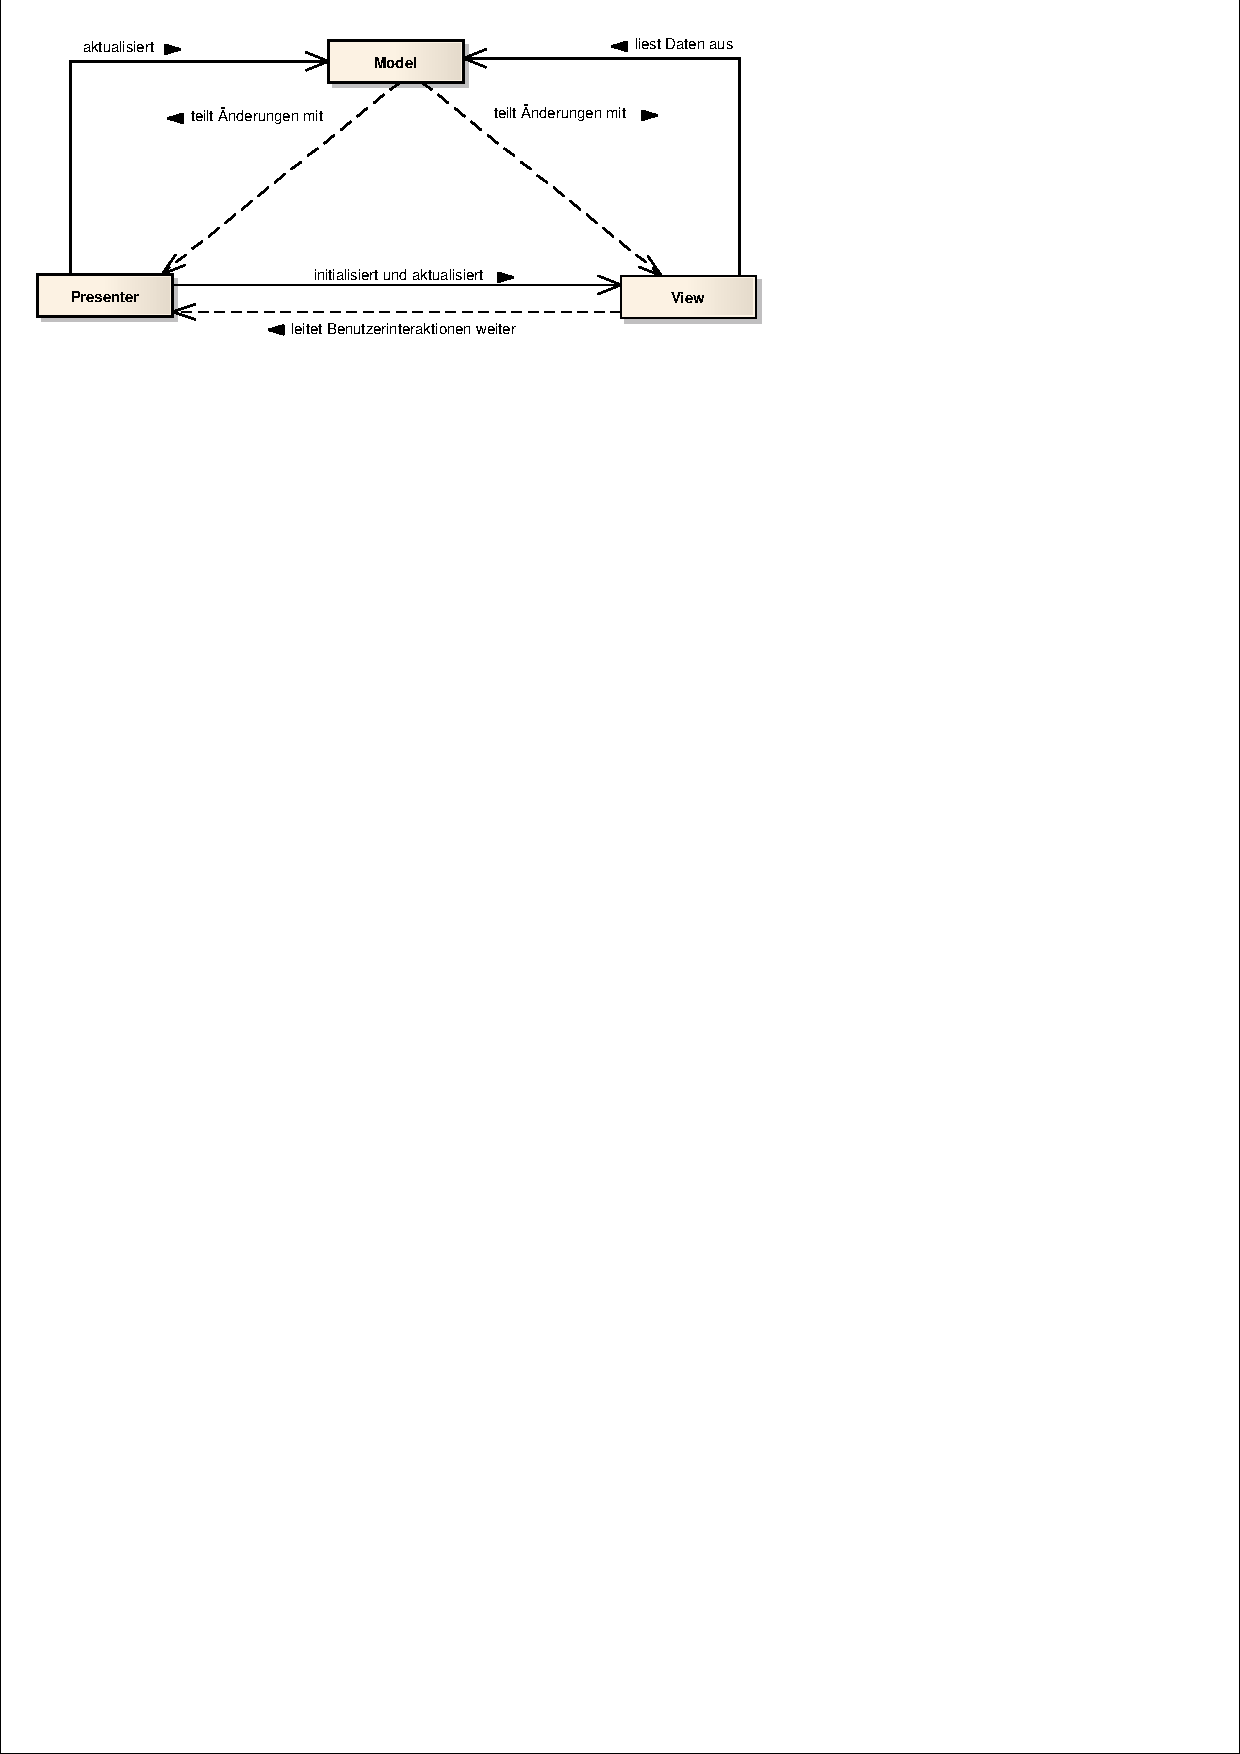
\includegraphics[trim = 2mm 238mm 80mm 2mm, clip, scale=0.7]{images/MVP.pdf}
\caption{�berblick �ber die \emph{Supervising Controllers} Variante des \emph{MVP Patterns}}\label{fig:mvp}
\end{figure}

Abbildung~\ref{fig:mvp} zeigt die \emph{Supervising Controllers} Variante des \emph{MVP Patterns} \cite{fowler}, welche vom \DevEnv\ verwendet wird. Jeder \emph{Presenter} hat genau eine \emph{View} und umgekehrt. Der \emph{Presenter} kennt seine \emph{View} und kann diese jederzeit aktualisieren und auf deren Daten zugreifen. Die \emph{View} hingegen kennt ihren \emph{Presenter} nicht. Um die Benutzereingaben dennoch an den \emph{Presenter} weiterleiten zu k�nnen, werden \emph{Events} verwendet. Der \emph{Presenter} reagiert darauf und aktualisiert gegebenenfalls die Daten des Modells. 

Die \emph{View} erh�lt ihre Daten entweder vollst�ndig vom \emph{Presenter}, oder kann diese aus dem Modell auslesen. �ndert sich das Modell, so werden die �nderungen �ber \emph{Events} sowohl an den \emph{Presenter} als auch an die \emph{View} geschickt. Im Regelfall bindet sich die \emph{View} per \emph{Databinding} an das Modell und wird so -- ohne zus�tzlichen Code -- automatisch aktualisiert, wenn sich das Modell �ndert. Der \emph{Presenter} kann ebenfalls auf �nderungen des Modells reagieren, um komplexere Pr�sentationslogik auszuf�hren und dann die \emph{View} zu aktualisieren. 

\section{System-Architektur}
In der ersten Iteration der Design-Phase wurde bereits die gesamte Architektur des \DevEnvs\ entworfen. Der erste Entwurf erwies sich als recht stabil und erforderte in sp�teren Iterationen nur wenige Modifikationen. Die erstellten Artefakte, ein Designmodell und mehrere Sequenzdiagramme, werden in den folgenden Abschnitten besprochen und die getroffenen Entscheidungen begr�ndet. Das Designklassen-Diagramm ist allerdings zu gro�, um es im Anhang dieser Arbeit abzubilden. Daher werden nur relevante Ausschnitte des Modells im Anhang beigelegt; das komplette Modell ist als .pdf-Datei auf der CD-ROM enthalten.

Da UML keine Syntax f�r .NET \emph{Properties} anbietet, wurde der Stereotyp \texttt{property} eingef�hrt. In der Implementierung wurden dann \texttt{Get/SetX}-Methoden mit \texttt{property}-Stereotyp als entsprechende \emph{Properties} \texttt{X \{ get; set; \}} umgesetzt. Aus Gr�nden der �bersichtlichkeit wurden im Designmodell f�r viele �ffentliche Attribute keine \emph{Properties} definiert; sie werden sp�ter aber als �ffentliche \emph{Properties} implementiert, da laut den .NET Richtlinien der Zugriff auf �ffentliche Klassenattribute immer durch \emph{Properties} gekapselt sein sollte \cite{fields}.

\subsection{\Horde-Klassen}
Die aus dem Konzeptmodell bekannten \Horde-Klassen wurden in das Designmodell �ber-nommen; alle Klassenattribute, die Assoziationen zwischen den Klassen und die Vererbungshierarchien sind unver�ndert. Es wurden allerdings mehrere Funktionen erg�nzt. So erh�lt die abstrakte Klasse \texttt{SceneNode} die virtuelle Methode \texttt{InitializeFromHorde3DState}, die aus dem aktuellen \Horde-Zustand beispielsweise die Transformationswerte und den Vaterknoten ausliest. Alle abgeleiteten Klassen k�nnen diese Methode �berschreiben, um ihre eigenen Daten auszulesen. Dabei k�nnen sie auf die \texttt{SceneNode}-Implementierung zur�ckgreifen, um die von \texttt{SceneNode} geerbten Attribute und Assoziationen zu f�llen beziehungsweise aufzubauen.

Ein analoges Vorgehen wurde f�r die Ressourcen-Hierarchie angewandt. Die abstrakte Klasse \texttt{Resource} besitzt ebenfalls eine virtuelle Methode \texttt{InitializeFromHorde3DState}, die in ihrer Standardimplementierung die \texttt{Resource}-Attribute und -Assoziationen ausliest und von den Subklassen �berschrieben werden sollte. Die Klasse \texttt{EditableResource} f�hrt zwei weitere abstrakte Methoden ein: \texttt{SaveToDisk} und \texttt{LoadFromDisk}. Konkrete Subklassen m�ssen diese Funktionen so implementieren, dass ihre Attribute und Assoziationen in das \Horde-XML-Format �bersetzt werden, beziehungsweise aus diesem ausgelesen und aufgebaut werden. Jedoch k�nnen manche Assoziationen nur dynamisch aus dem aktuellen \Horde-Zustand ermittelt werden, da sie in den XML-Dateien nicht gespeichert sind.

\subsection{Client-Server-Schnittstelle}
Wie bereits in Abschnitt~\ref{decisions} ausgef�hrt, zerf�llt das System in einen Client- und einen Serverteil. Da in der Design-Phase bereits die Windows Communication Foundation (WCF) als Netzwerk-Framework ausgew�hlt wurde, orientiert sich das Design der Client-Server-Schnittstelle an der Terminologie und an den F�higkeiten von WCF. 

Abbildung~\ref{fig:clientServerInterfaceDesign} zeigt einen Ausschnitt aus dem Designmodell f�r die Client-Server-Schnitt-stelle. Zun�chst wurde das Interface \texttt{IDebuggerService} spezifiziert, �ber das der Client auf den Server zugreifen kann. Der Service hat je eine Funktion f�r jede Systemanforderung: \texttt{Suspend} und \texttt{Resume}, um die Anwendung anzuhalten und wieder fortzusetzen; \texttt{Profile}, um die Profiling-Daten zu generieren; \texttt{GetRenderTargetData}, um den Inhalt eines \emph{Render Targets} auszulesen; und \texttt{UpdateResource}, um aktualisierte Ressource-Daten zu �bermitteln und an \Horde\ weiterzureichen.

Urspr�nglich lieferten die Funktionen bereits die jeweilig ben�tigten Daten zur�ck. %, was jedoch zu Deadlocks und Inkonsistenzen bei der Implementierung f�hrte\footnote{Die Deadlocks konnten entstehen, wenn w�hrend einer WCF-Operation weitere Benutzereingaben bearbeitet wurden. Da die WCF-Aufrufe sowohl client- als auch serverseitig immer in einem speziellen Thread stattfinden m�ssen.}. 
In der zweiten Iteration wurde hingegen das \texttt{IDebuggerServiceCallback}-Interface eingef�hrt. Der Server verwendet dieses Interface, um dem Client Daten und Ereignisse zu �bermitteln. Das \emph{Callback}-Interface vereinfachte das Einfrieren, Fortsetzen und Profilen der Anwendung aus der Anwendung selbst heraus. Wenn der Benutzer eine bestimmte Taste innerhalb der Anwendung dr�ckt, schickt der Server per \emph{Callback} eine Meldung an den Client, und dieser kann darauf entsprechend reagieren. Ohne \emph{Callbacks} w�re das in Sequenzdiagramm~\ref{fig:ClientServerCommunication} gezeigte Vorgehen nicht umsetzbar gewesen. Dort werden die \emph{Service}- und \emph{Callback}-Interaktionen beim Anhalten der Anwendung gezeigt. Der Client erh�lt vom Benutzer den Befehl zum Anhalten der Anwendung und ruft den \emph{Service} auf, welcher wiederum den Server informiert. Alternativ erteilt der Benutzer den Befehl durch einen Tastendruck innerhalb Anwendung direkt an den Server. In beiden F�llen ruft der Server die \texttt{OnSuspended}-Methode des \emph{Callbacks} auf. Eine Implementierung des \emph{Callback}-Interfaces w�rde den Client beispielsweise durch Ausl�sen eines \emph{Events} dar�ber informieren, dass die Anwendung angehalten wurde; der Client geht bis zu diesem Zeitpunkt in beiden F�llen immer noch davon aus, dass die Anwendung noch l�uft. Kam der \texttt{Suspend}-Aufruf direkt vom Server, so kann der Client davon nichts wissen. Kam der Aufruf hingegen vom Client selbst, so wurde er nur an den Server weitergereicht, aber sonst nicht darauf reagiert. Dadurch kann der Client unabh�ngig vom Ursprung des \texttt{Suspend}-Befehls die gleichen Aktionen durchf�hren. 

Erst wenn der Client durch den \emph{Callback} �ber das Einfrieren der Anwendung informiert wurde, fordert er mit der \texttt{RequestDebugData}-Methode des \emph{Services} die aktuellen Szenen\-graph- und Ressourcendaten an. Der Server schickt dann jede \emph{Scene Node} und jede Ressource einzeln �ber das \emph{Callback} Interface an den Client, der mit den Objekten entsprechend weiterarbeitet. Beim Fortsetzen oder Profilen der Anwendung w�re das Verfahren analog, es w�rden nur andere beziehungsweise gar keine Daten per \emph{Callback} an den Client zur�ckgeschickt werden. Eine Ausnahme bildet hingegen das Auslesen des Inhalts eines \emph{Render Targets}. Da die Anfrage ausschlie�lich vom Client kommen kann, bringt das \emph{Callback}-Verfahren hier keine Vorteile. Aus diesem Grund liefert die Funktion \texttt{GetRenderTargetData} das Ergebnis direkt zur�ck.

Ein weiterer Vorteil des \emph{Callback}-Interfaces ist die M�glichkeit, generierte \Horde-Mel\-dungen unverz�glich an den Client schicken zu k�nnen. Dies erspart ein kontinuierliches Nachfragen des Clients beim Server, ob neue Nachrichten erstellt wurden. Zus�tzlich werden alle \emph{Scene Nodes}, Ressourcen, \Horde-Meldungen und Profiling-Objekte einzeln �bertragen, was bei gro�en Datenmengen die Reaktionszeit des Clients verbessert. Statt auf die �bertragung des gesamten Datensatzes warten zu m�ssen, kann der Client nach und nach jedes Objekt, das er bereits erhalten hat, einzeln darstellen. 

Problematisch an der Einf�hrung des \emph{Callback}-Interfaces war hingegen, dass es prinzipiell m�glich sein k�nnte, dass \emph{Callbacks} vor dem Verbindungsaufbau aufgerufen werden. Aus diesem Grund stellt die Implementierung einen Sicherungsmechanismus bereit, der \emph{Callback}-Aufrufe abf�ngt und erst dann an den Client �bermittelt, wenn die Verbindung aufgebaut wurde.

Auf der Clientseite kennt nur die Klasse \texttt{Horde3DApplication} eine Instanz der Klasse \texttt{DebuggerServiceProxy}, �ber die der Client mit dem Server kommunizieren kann. Dabei repr�sentiert \texttt{Horde3DApplication} wie bereits im Konzeptmodell eine konkrete \Horde-Anwendung. Um eine Anwendung starten zu k�nnen, werden gewisse Informationen ben�tigt, wie der Pfad zur ausf�hrbaren Datei, die \emph{Endpoint}-Konfiguration f�r WCF, das Arbeitsverzeichnis etc. \texttt{Horde3DApplication} kennt diese Daten und die Methode \texttt{Start} startet eine neue Serverinstanz. Sobald der Server l�uft, dient die Klasse als Fassade f�r den Service \emph{Proxy}. Zum Beenden des Servers muss die Methode \texttt{ShutDown} aufgerufen werden.

\subsection{Umsetzung des DLL-Replacements und des Profilings}
Der gew�hlte DLL-\emph{Replacement}-Mechanismus macht die Einf�hrung von \emph{Proxy}-Funktionen erforderlich. Wenn die Anwendung eine \Horde-Funktion aufruft, so wird nicht sofort der Code der originalen \Horde\ DLL ausgef�hrt, sondern eine \emph{Proxy}-Funktion. Diese ruft die urspr�ngliche Funktion auf, f�hrt aber auch noch zus�tzlichen Code aus. Dieser Code h�ngt jedoch davon ab, ob der Server gerade die \Horde-Funktionsaufrufe f�r die Profiling-Funktion protokolliert. 

Um mit den unterschiedlichen Codepfaden zurechtzukommen, wurden die in Abbildung~\ref{fig:proxyDesign} gezeigte Klassenstruktur entworfen. \texttt{Horde3DProxyBase} ist eine abstrakte Basisklasse, die f�r jede \Horde-Funktion einen Funktionszeiger sowie eine gleichnamige, abstrakte Methode mit gleichen R�ckgabe- und Parametertypen wie die \Horde-Funktion besitzt. Aus Gr�nden der �bersichtlichkeit sind im Klassendiagramm~\ref{fig:proxyDesign} nur der Funktionszeiger und die \emph{Proxy}-Funktion f�r \texttt{Horde3D::getVersionString} eingezeichnet.

Die beiden Klassen \texttt{Horde3DNoProfilingProxy} und \texttt{Horde3DProfilingProxy} spezialisieren \texttt{Horde3DProxyBase}. Alle Funktionszeiger der Basisklasse werden geerbt und durch die ebenfalls geerbte \texttt{Initialize}-Methode initialisiert. Die beiden \emph{Proxy}-Klassen �berschreiben die abstrakten \Horde-Methoden: Es wird jeweils die urspr�ngliche \Horde-Funktion sowie die entsprechende Methode der statischen \texttt{Horde3DCall}-Klasse aufgerufen und gegebenenfalls die Profiling-Daten protokolliert. \texttt{Horde3DCall} besitzt f�r jede \Horde-Funktion eine statischen Methode und ein statisches \emph{Event}, welche jeweils die an die Funktion �ber\-ge\-benen Parameter und deren R�ckgabewert als Parameter erhalten. Wird eine \Horde-Methode der \texttt{Horde3DCall}-Klasse aufgerufen, so wird das entsprechende spezifische \emph{Event} sowie die beiden generischen \emph{Events} \texttt{Before-/AfterFunctionCalled}  ausgel�st, wobei letztere jeweils vor -- respektive nach -- dem Ausl�sen des speziellen Ereignisses ausgel�st werden. Objekte des Servers k�nnen sich an diesen \emph{Events} registrieren und werden somit informiert, wann und mit welchen Parameter- und R�ckgabewerten eine \Horde-Funktion aufgerufen wurde.

Die \texttt{Horde3DProxyHandler}-Klasse verwaltet die zwei verschiedenen \emph{Proxies} und h�lt eine Referenz auf die originale \Horde\ DLL, mit der die Funktionszeiger auf die \Horde-Funktionen ermittelt werden k�nnen. Mit \texttt{Initialize} werden die beiden \emph{Proxy}-Klassen initialisiert und eine Instanz des \texttt{Horde3DNoProfilingProxy} als Wert der \texttt{CurrentProxy}-Assoziation gesetzt. Die Methode \texttt{EnableProfiling} (de)aktiviert den Profiling-Modus, indem die \texttt{CurrentProxy}-Assoziation auf den entsprechenden \emph{Proxy} gesetzt wird.

Die API von \Horde\ verwendet allerdings keine Klassen, sondern organisiert die Funktionen im Namensraum \texttt{Horde3D}. Die \emph{Replacement}-DLL ben�tigt daher neben dieser Klassenstruktur noch \emph{Proxy}-Funktionen f�r alle \Horde-Funktionen im Namensraum \texttt{Horde3D} und eine globale Instanz der \texttt{Horde3DProxyHandler}-Klasse. Die \emph{Proxy}-Funktionen k�nnen dann mit der \texttt{GetCurrentProxy}-Methode der \texttt{Horde3DProxyHandler}-Klasse auf den derzeitigen \emph{Proxy} zugreifen und die entsprechende \Horde-Methode des \emph{Proxies} aufrufen. Dieser Vorgang wird am Beispiel des Profiling-\emph{Proxies} f�r die \Horde-Funktion \texttt{getVersionString} in Abbildung~\ref{fig:proxySeq} gezeigt, wobei zus�tzlich noch \texttt{FunctionCall}-Objekte f�r die Profiling-Funktionalit�t erzeugt werden.

Das beschriebene Design wurde gew�hlt, weil es eine klare Trennung zwischen den beiden verschiedenen \emph{Proxies} erm�glicht. Die Trennung wurde n�tig, da der Profiling-\emph{Proxy} f�r jeden Funktionsaufruf einige zus�tzliche Schritte durchf�hren und mehrere Objekte anlegen muss, was einen negativen Einfluss auf die Performance in CPU-limitierten Szenen hatte. Daher sollte der Profiling-Code, wenn er nicht ben�tigt wird, auch nicht ausgef�hrt werden. 

Es h�tte zwei denkbare Alternativen zur umgesetzten L�sung gegeben:

\begin{itemize}
	\item Man h�tte direkt in den \emph{Proxy}-Funktionen im \texttt{Horde3D}-Namensraum die Original-Funktionen aufrufen und den zus�tzlichen Code ausf�hren k�nnen, wobei man per \texttt{if-then-else} den Profiling-Code ein- und ausgeschaltet h�tte. Dadurch h�tte man sich den Aufruf der \texttt{GetCurrentProxy}-Methode gespart -- der aber im Regelfall vom Compiler sowieso \emph{inline} kompiliert wird -- und den virtuellen \Horde-Methodenaufruf des \emph{Proxies} durch die Auswertung einer Bedingung ersetzt. Der Performancevorteil der \texttt{if-then-else}-L�sung, falls �berhaupt messbar, w�re aber im Vergleich zur Aus\-f�hr\-ungs\-dauer der eigentlichen Funktionen so gering, dass statt dieser L�sung die im objekt-orientierten Sinne bessere Alternative gew�hlt wurde.
	
	\item Eine weitere Variante betrifft die \texttt{Horde3DCall}-Klasse. Diese bietet neben den beiden generischen \emph{Events}, die nur den Namen der aufgerufenen Funktion �bergeben, ein spezielles Ereignis mit Ein- und Ausgabewerten f�r jede \Horde-Funktion. Dies erfordert viel Code, der durch die Beschr�nkung auf die generischen \emph{Events} vermieden werden k�nnte. Dann m�sste man allerdings die Ein- und Ausgabewerte der aufgerufenen Funktionen als \texttt{Object}-\emph{Array} �bergeben. Das f�hrt aber bei jedem Funktionsaufruf zur Erzeugung vieler tempor�rer Objekte, erfordert \emph{Boxing} und \emph{Unboxing} f�r Parameter primitiver Datentypen und beim Zugriff auf das Parameter-\emph{Array} eine �berpr�fung der \emph{Array}-Grenzen sowie des Parametertyps. Da diese L�sung unperformant, belastend f�r den \emph{Garbage Collector} und zudem nicht einmal typsicher ist, wurde die aufw�ndigere, aber elegantere Variante gew�hlt.
\end{itemize}

\subsection{Anhalten der Anwendung}
In der ersten Iteration der Design-Phase war nicht klar, wie das Anhalten der Anwendung technisch genau l�sbar ist. Es wurde daher das \emph{Strategy Pattern} verwendet, um verschiedene Ans�tze m�glichst einfach ausprobieren und austauschen zu k�nnen. Abbildung~\ref{fig:suspendStrategyDesign} zeigt den relevanten Ausschnitt des Designmodells. Das Interface \texttt{ISuspendApplicationStrategy} stellt die beiden Funktionen \texttt{Suspend} und \texttt{Resume} bereit, nach deren Ausf�hrung die Anwendung entweder angehalten ist oder weiterl�uft. Bei der Implementierung zeigte sich, dass insgesamt drei verschiedene Strategien zum Anhalten der Anwendung ben�tigt werden: \texttt{StopTimeSuspendStrategy}, um der Anwendung ein Anhalten der Zeit vort�uschen zu k�nnen; \texttt{CursorSuspendStrategy}, um der Anwendung die Kontrolle �ber den Mauszeiger gezielt entziehen und wieder zur�ckgeben zu k�nnen; und \texttt{WndProcSuspendStrategy}, um das \emph{Window Procedure} der Anwendung ersetzen und damit Benutzereingaben �ber Maus und Tastatur abfangen zu k�nnen. Die Umsetzung dieser Strategien und ihre Probleme werden in Kapitel~\ref{suspendApp} genauer erl�utert.

Um diese Objekte nicht einzeln verwalten zu m�ssen, wurde in einer sp�teren Iteration die Container-Klasse \texttt{SuspendApplicationStrategy} hinzugef�gt, die ebenfalls vom \emph{Suspend}-Interface erbt. Einzige Aufgabe dieser Klasse ist es, beim Aufruf ihrer \texttt{Suspend}- und \texttt{Resume}-Methoden die entsprechenden Methoden aller Objekte im \texttt{Strategies}-\emph{Property} aufzurufen. In Kapitel~\ref{Ausblick} findet sich ein Vorschlag, wie man aufbauend auf dieser Instanz des \emph{Strategy Patterns} und der \texttt{SuspendApplicationStrategy}-Klasse eine weitere Strategie zum Anhalten der Anwendung integrieren k�nnte.

\subsection{Starten und Beenden des Servers}
Die Abbildungen~\ref{fig:startSeq} und~\ref{fig:DebuggerInitSeq} zeigen, was beim Starten des Servers nach Aufruf der \texttt{Start}-Methode der \texttt{Horde3DApplication}-Klasse geschieht. Zun�chst muss die originale \Horde\ DLL im Anwendungsverzeichnis umbenannt werden. Dann werden die ben�tigten DLLs des \DevEnvs\ in das Anwendungsverzeichnis kopiert, einschlie�lich der modifizierten \Horde\ DLL mit den \emph{Proxy}-Funktionen. Anschlie�end wird die Konfigurationsdatei f�r den Server generiert, die ebenfalls in das Anwendungsverzeichnis kopiert wird. Dannach wird der Prozess gestartet. Da es in der modifizierten \Horde\ DLL eine globale \texttt{Horde3DProxyHandler}-Variable gibt, wird beim Starten der Anwendung und nach dem Laden der modifizierten DLL automatisch eine \emph{Proxy Handler}-Instanz erzeugt. Der Konstruktor ruft die \texttt{Initialize}-Methode auf, die wiederum zun�chst den \texttt{Horde3DDebugger}-\emph{Singleton} initialisiert. Clientseitig wird sofort eine Instanz des \texttt{DebuggerServiceProxy} erzeugt und mit dem Verbindungsaufbau zum Server begonnen. Da es keine M�glichkeit gibt, vom Server �ber den Abschluss der Initialisierung informiert zu werden, wird einfach so lange ein Verbindungsaufbau versucht, bis der Serverprozess hochgefahren und initialisiert ist und die Verbindung erfolgreich aufgebaut werden konnte.

Auf der Serverseite werden Instanzen der beiden \Horde-\emph{Proxies} erzeugt und der Pro\-fil\-ing-Modus standardm��ig deaktiviert. Die Initialisierungsroutine des \texttt{Horde3DDebugger}-\emph{Single\-tons} liest zun�chst die Konfigurationsdaten aus der \emph{Settings}-Datei ein und �berpr�ft die \Horde-Version. Der gew�hlte DLL-\emph{Replacement}-Mechanismus macht es erforderlich, dass die Anwendung und der Server die gleiche Version von \Horde\ verwenden. Sollte das nicht der Fall sein, wird sich die Anwendung in vielen F�llen mit einer Windows-Fehler\-mel\-dung "`Prozedureinsprungspunkt "`\textit{ProzedurName}"' wurde in der DLL "`\Horde.dll"' nicht gefunden."' beenden, bevor der Server initialisiert wird. Es gibt aber auch F�lle, in denen Windows die fehlenden oder zus�tzlichen Einsprungspunkte nicht entdeckt. Dann �berpr�ft der Server anhand der \Horde-Versionskennung beider DLLs, ob unterschiedliche Versionen vorliegen. Sind die Versionen unterschiedlich, wird die Anwendung mit einer Fehlermeldung beendet.

Der \texttt{Horde3DDebugger}-\emph{Singleton} erzeugt neben der \texttt{DebuggerService}-Instanz noch zwei weitere Objekte: \texttt{Horde3DMessagesHandler} und \texttt{Horde3DStateWatcher}. Die Aufgabe des \texttt{Horde3DMessagesHandler}s ist es, nach jedem Funktionsaufruf eventuell neu generierten Meldungen abzufangen. Wurde eine oder mehrere Meldungen generiert, so werden die Daten ausgelesen, f�r jede neu generierte Nachricht ein \texttt{Horde3DMessage}-Objekt erzeugt und dieses per \emph{Callback} an den Client gesendet. 

Zu beachten ist hierbei die Phase der Initialisierung und Deinitialisierung des Servers. Der \texttt{Horde3DMessagesHandler} darf nur nach neuen Meldungen fragen, solange \Horde\ korrekt initialisiert ist. Wird beispielsweise \texttt{Horde3D::getVersionString} vor dem Aufruf von \texttt{Horde3D::init} aufgerufen, w�rde ohne korrekte \Horde-Initialisierung bereits nach dem Aufruf von \texttt{Horde3D::getVersionString} nach neuen Nachrichten gefragt. Auch nach dem Aufruf von \texttt{Horde3D::release} w�rde nach neuen Meldungen gefragt werden; zu diesem Zeitpunkt ist \Horde\ allerdings bereits vollst�ndig deinitialisiert. In beiden F�llen k�nnte es zu einem Absturz des Programms kommen.

Es ist allerdings kein Problem, wenn bereits Meldungen erzeugt werden, bevor der Client die Verbindung zum Server aufgebaut hat. Alle \emph{Callback}-Aufrufe werden abgefangen und erst ausgef�hrt, wenn die Verbindung steht.

Die \texttt{Horde3DStateWatcher}-Klasse hat derzeit nur die Aufgabe, unerw�nschtes \emph{Reverse-Engineering} zu unterbinden. Die Klasse k�nnte aber in Zukunft erweitert werden, um beispielsweise die Kamera, mit der die Szene gezeichnet wurde, zu protokollieren. Das k�nnte in Szenen mit mehreren Kameras und mehreren Aufrufen von \texttt{Horde3D::render} wichtig sein. Momentan �berpr�ft die Klasse allerdings nur, ob vor dem Aufruf von \texttt{Horde3D::render} die \Horde-Funktion \texttt{checkExtension} mit dem Parameter \texttt{AllowDebugging} aufgerufen wurde. Ist dies nicht der Fall, so wird beim Versuch die Szene zu zeichnen eine Fehlermeldung angezeigt und der Server beendet.

Das Beenden des Servers ist im wesentlichen eine Umkehr des Startprozesses. Die \texttt{ShutDown}-Methode der \texttt{Horde3DApplication}-Klasse schlie�t zun�chst die Verbindung zum Server und beendet den Prozess durch Schlie�en des Hauptfensters. Falls der Prozess nach einem kurzen \emph{Timeout} von wenigen Sekunden nicht beendet wurde, wird er zwangsweise terminiert. Anschie�end wird der urspr�ngliche Zustand des Anwendungsverzeichnis wiederhergestellt. Die in das Verzeichnis kopierten DLLs des \DevEnvs\ werden gel�scht und auch die erstellte Konfigurationsdatei wird entfernt. Zum Schluss wird der umbenannten, originalen \Horde\ DLL wieder ihr urspr�nglicher Name gegeben.

\subsection{Aktualisieren von Ressourcen-Daten}
Das Sequenzdiagramm~\ref{fig:UpdateResourceSeq} stellt das Vorgehen f�r die Aktualisierung von ge�nderten Ressourcen dar. Der Vorgang wird �ber die \texttt{Horde3DApplication}-Klasse angesto�en, da nur diese Klasse die \texttt{UpdateResource}-Operation des Servers aufrufen kann. Der Server f�hrt die interne \texttt{UpdateHorde3D}-Methode der �bergebenen \texttt{EditableResource} aus. Diese Methode ist virtuell und kann somit von den Subklassen �berschrieben werden. Das Sequenzdiagramm zeigt die Funktionsweise der Stand\-ard\-implementierung. Zun�chst wird �berpr�ft, ob die Ressource, die \Horde\ gerade unter dem gleichen \texttt{ResHandle} kennt, den gleichen Typ und gleichen Namen hat. Implizit wird damit auch �berpr�ft, ob �berhaupt noch eine Ressource mit diesem \texttt{ResHandle} existiert. Dies ist notwendig, weil es das \DevEnv\ erlaubt, die Anwendung nach dem Einfrieren der Szene und nach dem Auslesen der bekannten Ressourcen weiter auszuf�hren. Der Benutzer k�nnte nun eine Ressource bearbeitet haben und diese an die \texttt{UpdateResource}-Operation des Servers �bergeben. Zwischenzeitlich k�nnte die Anwendung die Ressource aber gel�scht und ihren \texttt{ResHandle} neu vergeben haben. Durch die �berpr�fung des Ressourcennamens und -typs soll verhindert werden, dass die �bergebene Ressource eine eventuell neu hinzugef�gte Ressource �berschreibt. Ansonsten w�rde die derzeit geladene Ressource durch eine eventuell v�llig andere ersetzt. Bei unterschiedlichen Typen w�rde \Horde\ eine Fehlermeldung erzeugen, da die �bergebenen Ressourcen-Daten dann nicht korrekt interpretiert werden k�nnen.

Ist die �berpr�fung jedoch erfolgreich, werden die derzeit geladenen Ressourcen-Daten gel�scht. Die Ressource selbst bleibt aber erhalten, insbesondere �ndert sich ihr \texttt{ResHandle} nicht. Nun k�nnen die Daten aus der �bergebenen \texttt{EditableResource} in ein \texttt{byte}-\emph{Array} kopiert und an \Horde\ �bergeben werden. Anschlie�end werden alle zur Zeit nicht geladenen aber bekannten Ressourcen geladen. Das ist erforderlich, weil die aktualisierte Ressource auf neue, noch nicht geladene Ressourcen verweisen k�nnte. Bevor die Szene mit der aktualisierten Ressource gezeichnet werden kann, m�ssen diese Abh�ngigkeiten geladen werden.

Wie bereits erw�hnt ist die \texttt{UpdateHorde3D}-Methode der \texttt{EditableResource}-Klasse virtuell. Werden n�mlich Shader- oder Material-Ressourcen aktualisiert, m�ssen noch einige zus�tzliche Schritte ausgef�hrt werden. \Horde\ erlaubt das Klonen von Materials, das hei�t, die Material-Ressource wird kopiert und der Kopie ein neuer \texttt{ResHandle} zugewiesen. Dadurch k�nnen zum Beispiel die \emph{Uniform}-Parameter des Materials f�r verschiedene Objekte unterschiedlich gesetzt werden. Allerdings werden die Kopien nicht aktualisiert, wenn das Original-Material aktualisiert wird. �bergibt man also eine \texttt{MaterialResource} an \texttt{UpdateResource}, so m�ssen alle Kopien des Materials gesucht und aktualisiert werden. Die Kopien sind an ihrem Namen erkennbar: hie� das Original-Material \texttt{Material1.material.xml}, dann hei�en die Klone \texttt{Material1.material.xml|X}, wobei $X$ der \texttt{ResHandle} der Kopie ist.

Wird eine \texttt{ShaderResource} an \texttt{UpdateResource} �bergeben, m�ssen ebenfalls noch weitere Ressourcen aktualisiert werden. Der GLSL-Code des Shaders wird von \Horde\ in zus�tzlichen Code-Ressourcen gespeichert. Wird ein Shader aktualisiert, werden allerdings die Code-Ressourcen nicht automatisch neu geladen. Dies muss manuell geschehen. Dazu werden die abh�ngigen Code-Ressourcen �ber den Namen ermittelt, der als Pr�fix den Namen der zugeh�rigen Shader-Ressource enth�lt. Allerdings kann diese Sonderbehandlung der Shader-Ressourcen f�r zuk�nftigen \Horde-Versionen entfallen. Alle Versionen nach \Horde\ 1.0.0 Beta 3 aktualisieren automatisch auch alle abh�ngigen Code-Ressourcen.
\section{Anbindung der Benutzeroberfl�che an das System}
Die Anbindung der grafischen Benutzeroberfl�che an den Anwendungscode wurde bislang nicht weiter betrachtet, ist jedoch ein komplexes Problem. F�r das \DevEnv\ wurde eine eigene Bibliothek entwickelt, die die GUI-Anbindung an das System kapselt und einige Grundfunktionalit�ten bereitstellt. Dabei standen die Wiederverwendbarkeit der Bibliothek sowie eine saubere Trennung zwischen GUI- und Anwendungscode im Vordergrund. 

\subsection{Alternativen zur Eigenentwicklung eines GUI-Frameworks}
Bevor mit der Entwicklung eines eigenen GUI-Frameworks begonnen wurde, wurden zwei alternative Ans�tze in Betracht gezogen: Die Integration des Clients in Visual Studio oder in SharpDevelop\footnote{\url{http://www.icsharpcode.net/OpenSource/SD}} als Plugin. Beide Tools haben eine ausgereifte, m�chtige und bew�hrte Plugin-Architektur und bieten viele Schnittstellen zu Subsystemen -- wie einen Texteditor mit \emph{Syntaxhighlighting}, eine Konsole f�r Textausgabe, ein \emph{Undo}/\emph{Redo}-Framework, ein Framework zum automatischen Speichern ge�nderter Dateien, etc. --, die das \DevEnv\ ebenfalls ben�tigt. Es bestand also ein gro�es Potential, bereits vorhandene und erwiesenerma�en gut funktionierende L�sungen wiederzuverwenden. Dennoch wurde auf diesen Vorteil verzichtet, da die Nachteile �berwogen. Visual Studio ist ein extrem komplexes und im Kern auch sehr altes System, das zu weiten Teilen noch in \C++ und COM implementiert ist. Plugins k�nnen zwar in \Csharp/.NET entwickelt werden, allerdings sind die Interfaces, die Visual Studio bereitstellt, aufgrund ihres Alters �berladen, schwer verst�ndlich und nicht mehr zeitgem��. Au�erdem muss ein Plugin nach jeder �nderung neu integriert werden, was die Entwicklung verz�gert und ein schnelles Debuggen unm�glich macht. Ein weiteres Problem ist, dass nicht jeder potenzielle Benutzer des \DevEnvs\ eine Visual Studio Lizenz besitzt; die kostenlosen Express-Versionen unterst�tzen leider keine Plugins. Die eigenst�ndig lauff�hige Visual Studio Shell w�rde diese Probleme zwar l�sen, w�re aber aufgrund ihrer Gr��e (ca. 150 MByte) und Komplexit�t eine sehr belastende Abh�ngigkeit f�r das \DevEnv.

SharpDevelop hingegen wurde von Anfang an komplett in \Csharp\ entwickelt und ist Open Source. Die Einbindung von Plugins gestaltet sich angenehmer als unter Visual Studio und es gibt moderne objekt-orientierte APIs f�r den Zugriff auf die Standardkomponenten der Entwicklungsumgebung. Leider ist die Entwicklung von Plugins f�r SharpDevelop sehr schlecht dokumentiert. Es gibt zwar einf�hrende Erl�uterungen, aber eine prototypische Implementierung des \DevEnvs\ zeigte schnell, dass bei komplexeren Fragen und Problemen oft keine Hilfestellung in der Dokumentation, im Internet oder im inzwischen veralteten Buch \cite{sharpdevelop} existiert. Da die IDE Open Source ist, konnte die Antwort zwar immer durch Durchsehen des Quellcodes gefunden werden, dies nahm aber sehr viel Zeit in Anspruch. Visual Studio hingegen ist teilweise deutlich besser dokumentiert. Aber auch hier gibt es noch einige Defizite, insbesondere bei der Erweiterung der Standard-Projektverwaltung mit dem \emph{Visual Studio Managed Package Framework for Projects}\footnote{\url{http://www.codeplex.com/mpfproj}}.

\subsection{Architektur des GUI-Frameworks}\label{sec:aufbau}
Um eine klare Trennung zwischen GUI- und Anwendungscode zu erreichen, ist das GUI-Framework eine Instanz des \emph{Model-View-Presenter Patterns}. Es wurde au�erdem von Anfang an auf die Entwicklung einer Visual Studio-�hnlichen Oberfl�che ausgelegt, kann aber prinzipiell auch f�r andere UI-Designs verwendet werden. 

Abbildung~\ref{fig:guiClass} zeigt das Designklassen-Diagramm des GUI-Frameworks. Die Verwendung des \emph{Model-View-Presenter Patterns} wird durch die abstrakte Klasse \texttt{Presenter} und das Interface \texttt{IView} deutlich. Im GUI-Framework selbst kommen keine Modelle vor; diese sind anwendungsspezifisch und werden von den Applikationen, die das Framework verwenden, bereitgestellt.

Es gibt insgesamt vier Klassen, die das \texttt{IView}-Interface implementieren. Diese Klassen ergeben sich aus dem Design moderner GUI-Frameworks wie Windows Forms und der Windows Presentation Foundation. Dort gibt es zum einen \texttt{Form}-Klassen, welche ein eigenst�ndiges Fenster repr�sentieren. Diesen Fenstern k�nnen mehrere Instanzen von \texttt{UserControl}-Klassen untergeordnet sein, beispielsweise f�r Eingabefelder oder Schaltkn�pfe. Um das Visual Studio-�hnliche Design zu realisieren, gibt es noch eine weitere spezielle Klasse, \texttt{DockContent}, deren Instanzen ebenfalls einer \texttt{Form} untergeordnet sein m�ssen. Dabei kann eine \texttt{DockContent}-Instanz sowohl ein eventuell verstecktes \emph{Dock Pane} an der Seite der Oberfl�che, ein \emph{Floating Window} oder ein Dokument sein. F�r all diese Klassen wird eine \texttt{IView}-Implementierung ben�tigt. \texttt{UserControlView} erbt von \texttt{UserControl} und \texttt{FormView} ist von \texttt{Form} abgeleitet, wobei hier zwischen modalen und nicht-modalen Fenstern unterschieden wird. \texttt{DockView} erbt von \texttt{DockContent} und f�gt zwei Attribute hinzu, um den standardm��igen \texttt{DockState} und die Menge der erlaubten \texttt{DockState}s festzulegen. \texttt{DocumentView} ist eine Subklasse von \texttt{DockView}, wobei hier der standardm��ige \texttt{DockState} und die Menge der erlaubten \texttt{DockState}s fest auf \texttt{Document} beschr�nkt sind.

Die abstrakte Klasse \texttt{Presenter} ist die Basisklasse f�r alle \emph{Presenter} im System. Instanzen von \texttt{Presenter} werden �ber einen Namen identifiziert; f�r einen gegebenen Namen kann es immer nur eine \texttt{Presenter}-Instanz geben. \texttt{Presenter} hat eine private Assoziation zu einem \texttt{IView}, auf die abgeleitete Klassen nur �ber die Funktion \texttt{UpdateView} zugreifen k�nnen. Damit wird zum einen die Kopplung zur \emph{View} verringert und zum anderen m�ssen in dieser Funktion noch einige implementierungsspezifische Details (Zugriff �ber korrekten Thread, kein Zugriff auf bereits gel�schte \emph{Views}, etc.) geregelt werden. Zu beachten ist, dass nur die abstrakte \texttt{Presenter}-Klasse ihre zugeh�rige \emph{View} kennt; insbesondere kennen die \texttt{IView}-Instanzen nicht ihre zugeh�rige \texttt{Presenter}-Instanzen. Dies wird durch das \texttt{Request}-Ereignis, das alle \texttt{IView}-Implementierungen besitzen, erm�glicht. Ein \emph{Presenter} registriert sich an den \texttt{Request}-Ereignissen seiner \emph{View} und kann dar�ber �ber Eingaben und Aktionen des Benutzers informiert werden.

Die GUI-\emph{Controls} bilden eine Hierarchie aus \texttt{Form}-, \texttt{DockContent}- und \texttt{UserControl}-In\-stan\-zen. Diese Hierarchie m�ssen auch die \emph{Presenter} widerspiegeln. Aus diesem Grund kann ein \texttt{Presenter} einen \texttt{Parent} und beliebig viele \texttt{Children} haben, die �ber die Funktionen \texttt{Add-/RemoveChildPresenter} hinzugef�gt und wieder entfernt werden k�nnen. \texttt{Presenter} hat au�erdem abstrakte Methoden f�r die Initialisierung und Deinitialisierung. Abgeleitete \texttt{Presenter}-Klassen m�ssen diese Methoden mit einer speziellen Implementierung �ber\-schrei\-ben. Die \emph{Presenter}- und \emph{View}-Hierarchien  sind eine Instanz des \emph{Composite Patterns}.

Da eine \emph{Undo}/\emph{Redo}-Funktionalit�t ben�tigt wird, werden vom Benutzer ausgef�hrte Aktionen gem�� des \emph{Command Patterns} durch Objekte gekapselt, die von der abstrakten Klasse \texttt{Command} erben m�ssen. Ein \texttt{Command} hat Funktionen zum Ausf�hren der Aktion (\texttt{Execute}), sowie zum R�ckg�ngigmachen (\texttt{Undo}) und Wiederholen (\texttt{Redo}); wobei \texttt{Redo} standardm��ig einfach noch einmal \texttt{Execute} aufruft und \texttt{Execute} und \texttt{Undo} abstrakt sind. Es ist auch m�glich, die \emph{Undo}/\emph{Redo}-Funktionalit�t f�r einen \texttt{Command} zu deaktivieren, indem die \texttt{CanUndo}- und \texttt{CanRedo}-Attribute auf \texttt{false} gesetzt werden. Instanzen von \texttt{Command} werden immer von einem \texttt{Presenter} erzeugt und jeder \texttt{Command} kennt seinen Erzeuger. �ber diese Assoziation k�nnen alle \texttt{Command}-Objekte eines \texttt{Presenter}s beim Entfernen des \texttt{Presenter}s aus der GUI gel�scht werden, wodurch die Aktionen dieser \texttt{Command}s nicht mehr r�ckg�ngig gemacht werden k�nnen.

\texttt{Command}-Objekte werden vom \texttt{CommandDispatcher} verwaltet. Dessen \texttt{HandleCommand}-Me-thode ruft die \texttt{Execute}-Methode des �bergebenen \texttt{Command}s auf und verwaltet intern eine \emph{Undo}-/\emph{Redo}-Liste von bereits ausgef�hrten Aktionen. Der \texttt{CommandDispatcher} kann �ber die Funktionen \texttt{Undo} und \texttt{Redo} angewiesen werden, eine Aktion r�ckg�ngig zu machen oder zu wiederholen. Dies ist allerdings nur m�glich, wenn das \texttt{CanUndo}- respektive das \texttt{CanRedo}-Attribut des \texttt{CommandDispatcher}s auf \texttt{true} gesetzt ist. �ndert sich der Wert eines dieser Attribute wird ein entsprechendes Ereignis ausgel�st, ebenso nach dem R�ckg�ngigmachen und Wiederholen einer Aktion.

Das \DevEnv\ stellt editierbare Ressourcen als \texttt{DocumentView}-Instanzen dar. Nach dem �ndern einer Ressource sollen die �nderungen gespeichert werden k�nnen. Au�erdem soll das Framework einen visuellen Hinweis geben, falls ein Dokument ge�ndert wurde, aber die �nderungen noch nicht gespeichert sind. Schlie�t der Benutzer ein ge�ndertes und noch nicht gespeichertes Dokument, so soll das Framework den Benutzer fragen, ob die �nderungen gespeichert oder verworfen werden sollen. Diese Aufgaben �bernimmt die \texttt{SaveableContentManager}-Klasse, an der \texttt{Presenter}, die das \texttt{ISaveableContentPresenter}-Interface implementieren, registriert und wieder entfernt werden k�nnen. Registrierte \texttt{ISaveableContentPresenter}-Instanzen k�nnen einzeln oder alle auf einmal gespeichert werden. Wird ein ge�nderter, aber noch nicht gespeicherter \texttt{Presenter} geschlossen, so wird der Benutzer gebeten, die �nderungen zu speichern oder zu verwerfen.

Das \texttt{ISaveableContentPresenter}-Interface stellt Methoden zum Laden und Speichern des zu persistierenden Objekts bereit. Auch der aktuelle \texttt{SaveState} wird dort verwaltet. Das Interface wird von der abstrakten Klasse \texttt{SaveableContentPresenter} implementiert, die die normale \texttt{Presenter}-Klasse erweitert.

Die \texttt{Shell}-Klasse ist schlie�lich das Hauptelement des Frameworks. In ihr laufen alle Vorg�nge zusammen. \texttt{CommandDispatcher} und \texttt{SaveableContentManager} sind mit einer 1:1-Assoziation zur \texttt{Shell} verbunden und h�tten somit auch direkt in die \texttt{Shell}-Klasse integriert werden k�nnen. Dies h�tte jedoch zu einer niedrigen Koh�sion und damit zu einer �berladung der \texttt{Shell}-Klasse gef�hrt, was durch die Verteilung der Zust�ndigkeiten vermieden wurde. Da der \texttt{SaveableContentManager} nur der \texttt{Shell} bekannt ist, ist die \texttt{Shell} hier eine Instanz des \emph{Facade Patterns}. Auch das \emph{Singleton Pattern} wird von der \texttt{Shell} verwendet: Mit dem \texttt{Current}-Attribut kann global auf die \texttt{Shell}-Instanz zugegriffen werden, wobei es nur eine \texttt{Shell}-Instanz pro \emph{AppDomain} geben darf. Dies ist konsistent mit dem Vorgehen der \texttt{Application}-Klasse der Windows Presentation Foundation.

Die Aufgabe der \texttt{Shell}-Klasse ist neben der Initialisierung der gesamten Oberfl�che auch die Verwaltung aller \texttt{Presenter}-Instanzen. \texttt{Presenter} k�nnen hinzugef�gt, wieder entfernt und Dokumente einzeln oder gemeinsam gespeichert oder geschlossen werden. Auch das Layout der \emph{Dock Panes} wird von der \texttt{Shell}-Klasse automatisch persistiert und beim Starten der Anwendung wiederhergestellt.

\subsection{Identifizierung der ben�tigten Modelle}
Modelle tauchen in Abbildung~\ref{fig:guiClass} nicht auf, da das GUI-Framework kein Interface und keine Zugriffswege f�r Modelle vorgibt. Dies erm�glicht einem \emph{Presenter}-\emph{View}-Paar die Verwendung mehrere Modelle, wovon die Implementierung des \DevEnvs\ auch Gebrauch macht. Insgesamt werden zur Umsetzung der Systemanforderungen sechs Modelle ben�tigt, die im Designmodell mit dem Stereotyp \texttt{model} gekennzeichnet sind.

\begin{itemize}
	\item \texttt{\textbf{Horde3DApplication}}: Die \texttt{Horde3DApplication}-Klasse repr�sentiert die \Horde-An-wendung, in der gerade der Server l�uft oder die gestartet werden kann. Sie ist die einzige Zugriffsm�glichkeit auf Operationen des Servers.
	
	\item \texttt{\textbf{CallbackHandler}}: Der \texttt{CallbackHandler} nimmt die \emph{Callbacks} des Servers entgegen und generiert f�r jede Nachricht ein entsprechendes \emph{Event}. Die \emph{Presenter} k�nnen sich an der \texttt{CallbackHandler}-Instanz an verschiedenen Ereignissen registrieren, um �ber Server-Nachrichten informiert zu werden.
	
	\item \texttt{\textbf{MessagesDispatcher}}: Die Aufgabe des \texttt{MessagesDispatcher}-Modells ist die Verwaltung aller erzeugten Nachrichten. Die Nachrichten k�nnen zum einen aus der \Horde-Anwendung stammen oder vom Client generierte Fehler- oder Debugmeldungen sein. Die Nachrichten werden nach ihrer Herkunft (Client oder Server) kategorisiert und nach Wichtigkeit (Debug, Information, Warnung oder Fehler) unterschieden. Der \emph{Dispatcher} unterst�tzt auch das Entfernen aller Nachrichten einer bestimmten Kategorie. Nachdem Meldungen entfernt oder hinzugef�gt wurden, wird ein spezielles Ereignis ausgel�st, damit die interessierten \emph{Presenter} und \emph{Views} entsprechend reagieren k�nnen.
	
	\item \texttt{\textbf{SceneGraph}} und \texttt{\textbf{ResourceGraph}}: Diese beiden Modelle dienen zum Verwalten aller bekannten \emph{Scene Nodes} und Ressourcen. Werden neue Objekte eingef�gt oder Objekte entfernt, wird ein \texttt{GraphChanged}-\emph{Event} ausgel�st, um die �nderungen bekannt zu machen.
	
	\item \texttt{\textbf{ProfilingDataManager}}: Dieses Modell funktioniert �hnlich der beiden zuvor genannten Modelle und verwaltet die Profiling-Daten. Das \texttt{ProfilingDataChanged}-\emph{Event} wird ausgel�st, wenn Profiling-Daten empfangen oder gel�scht werden.
\end{itemize}

\begin{figure}[htp]
\centering
%trim=l b r t  	This option will crop the imported image by l from the left, b from the bottom, r from the right, and t  from the top. Where l, b, r and t are lengths. 
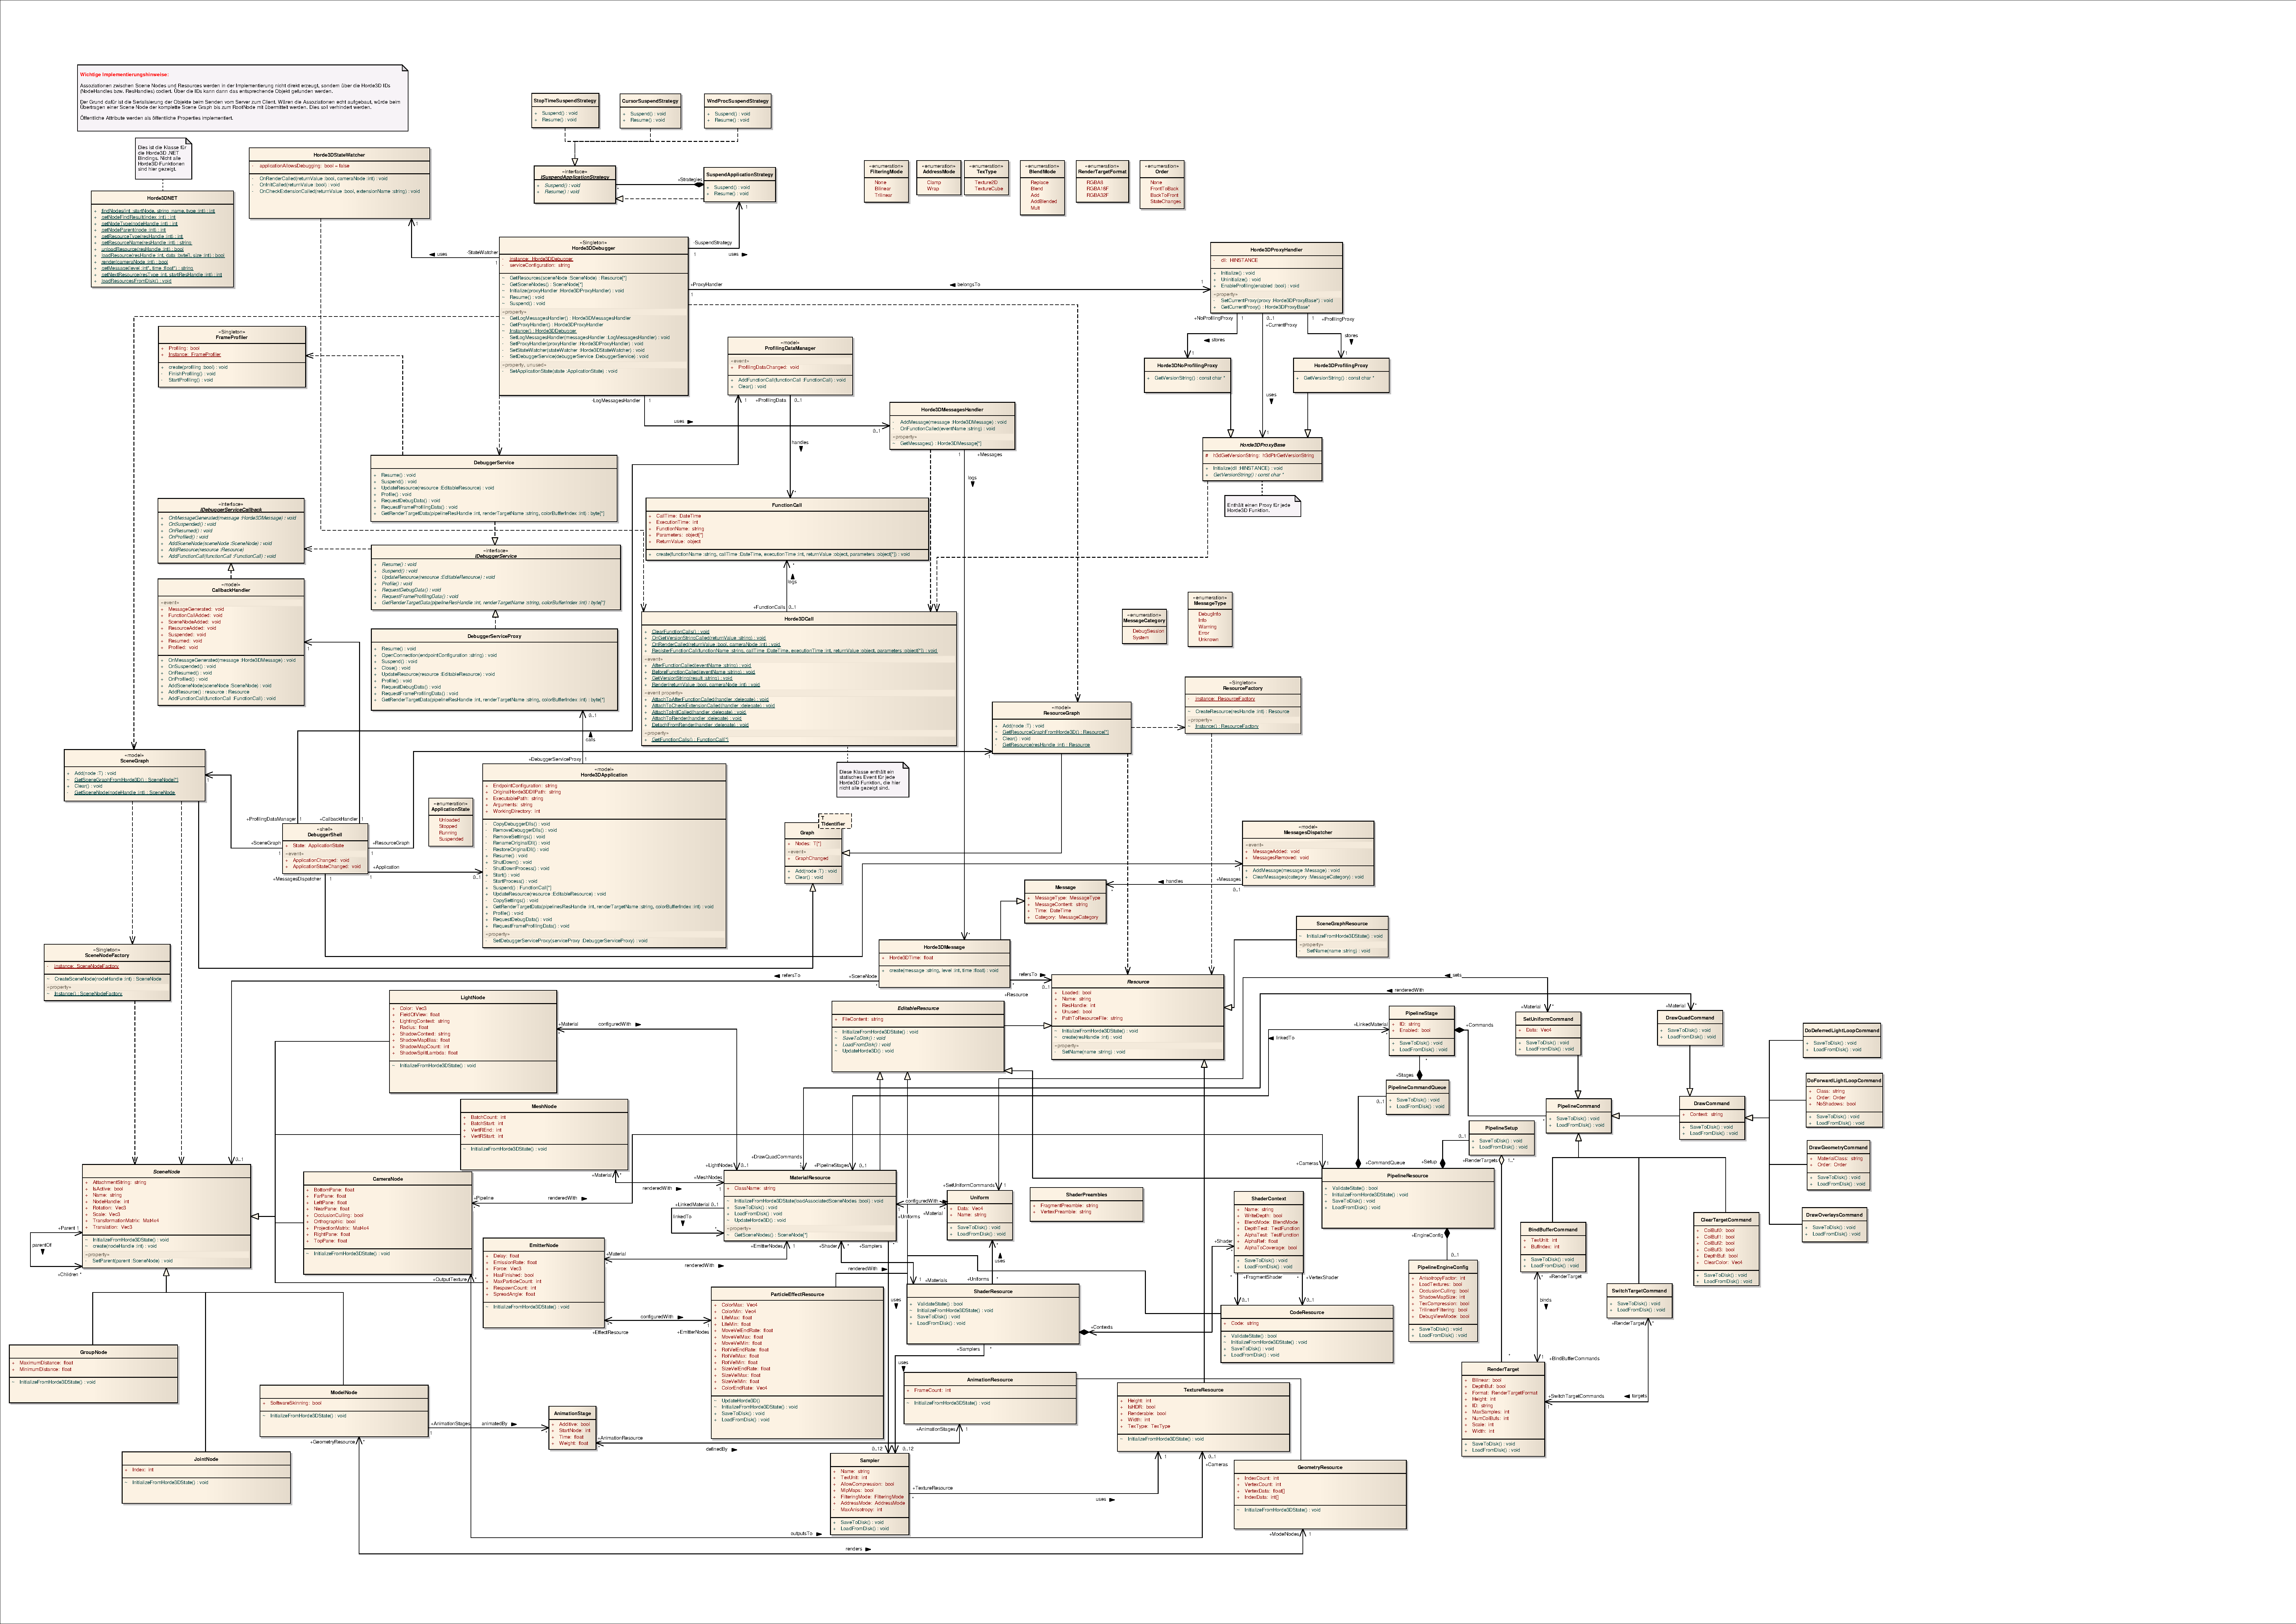
\includegraphics[trim = 125mm 380mm 975mm 415mm, clip, scale=0.7]{images/Designmodell.pdf}
\caption{Die Shell des \DevEnvs\ im Designmodell}\label{fig:shellDesign}
\end{figure}

Alle Modelle werden von der \texttt{Shell}-Klasse verwaltet, wodurch alle \emph{Presenter} Zugriff auf alle Modelle erhalten. Die \texttt{Shell}-Klasse �berwacht au�erdem den aktuellen Zustand des Servers, da einige \emph{Presenter} und \emph{Views} bei Zustands�nderungen spezielle Aktionen durchf�hren m�ssen. Die m�glichen Zust�nde sind \texttt{Unloaded}, wenn derzeit kein \texttt{Horde3DApplication}-Modell geladen ist und somit der Server nicht gestartet werden kann; \texttt{Stopped}, wenn der Server zur Zeit nicht l�uft aber gestartet werden kann; \texttt{Suspended}, wenn der Server gerade l�uft und die Szene eingefroren ist; und \texttt{Running} sonst. Die \texttt{Shell}-Klasse l�st ein \emph{Event} aus, sobald sich der Zustand des Servers �ndert.
\section{Konklusion}
In der Design-Phase wurden viele generische Konzepte verwendet, um flexibel auf m�gliche �nderungen von \Horde\ oder eventuell auftauchende Probleme in der Implementierungs-Phase reagieren zu k�nnen. Aufgrund der detaillierten Analyse der Anforderungen und dem Aufbau von \Horde\ konnte ein Systemdesign erstellt werden, das bei der Implementierung nur wenige Probleme verursachte. Die notwendigen �nderungen am Design beschr�nkten sich jedoch immer auf einzelne Klassen; die grundlegende Architektur blieb bestehen. Eine gr��ere �nderung ergab sich lediglich durch die Einf�hrung der Client-Server-\emph{Callbacks}. 

Im Rahmen dieser Bachelorarbeit wurde aber nicht das komplette Design implementiert. So gibt es gerade bei den \Horde-Klassen einige Attribute und Assoziationen, die zwar im Designmodell vorhanden sind, f�r die Umsetzung der Systemanforderungen aber nicht erforderlich waren. Sie wurden dennoch in das Konzept- und Designmodell aufgenommen, um die Modelle zu vervollst�ndigen. Im Code k�nnen diese bei Bedarf einfach hinzugef�gt werden.

Bei der Entwicklung des \DevEnvs\ wurde auch deutlich, dass der verwendete DLL-\emph{Replacement}-Mechanismus sowie die Einf�hrung der \texttt{Horde3DCall}-Klasse richtige Entscheidungen waren. Insbesondere die beiden Klassen \texttt{Horde3DMessagesHandler} und \texttt{Horde3DStateWatcher} zeigten, warum das Ausl�sen von generischen als auch spezifischen Ereignissen mit den genauen Aufrufsparametern und R�ckgabewerten nach einem \Horde-Funktionsaufruf sinnvoll ist. Diese Informationen sind f�r unterschiedlichste Aktionen n�tzlich; so wurde beim Entwurf dieses Verfahrens nicht an die Verwendung eines \emph{Reverse-Engineering}-Schutzes gedacht. Sowohl die \texttt{Horde3DStateWatcher}-Klasse als auch die Anforderung vor dem Schutz vor unerw�nschtem \emph{Reverse-Engineering} wurden erst in einer sp�teren Iteration ins \DevEnv\ aufgenommen und f�gten sich nahtlos in das Systemdesign ein.

Die Entwicklung des GUI-Frameworks war zeitaufw�ndig und h�tte vermieden werden k�n\-nen, wenn das \DevEnv\ als Plugin f�r Visual Studio oder SharpDevelop entwickelt worden w�re. Aufgrund verschiedener Unzul�nglichkeiten der Plugin-Infrastruktur der IDEs hat sich die Eigenentwicklung schlie�lich doch als die bessere L�sung herausgestellt, da sich w�hrend der Implementierung des Systems die St�rken des Frameworks zeigten und ein z�gige und unkomplizierte Umsetzung des Designs erm�glichten. So ist der GUI- und Anwendungscode stets klar voneinander abgegrenzt und es ist einfach, neue Features durch Implementieren weiterer \texttt{Presenter}- und \texttt{View}-Klassen hinzuzuf�gen. Die Wiederverwendbarkeit und Erweiterbarkeit des Frameworks konnte bereits im Rahmen der Bachelorarbeit �berpr�ft werden. So wurde zu einem sp�teren Zeitpunkt eine weitere \texttt{DockView}-Subklasse, \texttt{WpfDockView}, hinzugef�gt, mit der Windows Presentation Foundation \texttt{UserControl}s in Windows Forms \texttt{DockView}s dargestellt werden k�nnen. Der Einsatz des Frameworks bei der Entwicklung des Code Generators, siehe Abschnitt~\ref{CodeGen}, best�tigte die Wiederverwendbarkeit der Bibliothek.